\documentclass{article}
\usepackage{tikz}
\usepackage{darkmode}
\enabledarkmode
\author{Pierson}
\begin{document}
\title{Calc III Notes}

\maketitle

\section{Multivariable calc goals}
\begin{list}{-}{}
    \item vectors and geometry of R''
    \item functions of serval variables diff and int
    \item higher dimensional versions of FTC
    \item fund them for line integrals
    \item greens them
    \item stokes them
    \item divergence them
\end{list}

\setcounter{section}{11}
\section{Chapter 12: vectors and geo of space}
\subsection{}
    \begin{list}{-}{}
    \item \[R = line\] dist(x,y) = $ |y - x | $
    \item \[R^2 = Plane\] Orders pairs of (x,y) of real numbers
    \item \[R^3 = space\] ordered triples of (x,y,z) of real numbers
    \end{list}

right-hand rule: point fingers toward pos x-axis and curl towards pos y-axis, thumb should point to positive z\\


$R^n$ = n-tuples $(x_1, x_2, ... x_n)$ n-dim space\\

Distance D from (0,0) to (x,y)
\[D^2 = x^2 +y^2\]

Distance D from (0,0,0) to (x,y,z)
\[ D = \sqrt{x^2+yy^2+z^2}\] 

Sphere with center $X_0, Y_0, Z_0$ and radius R has equation:

\[ (X-X_0)^2 + (y-y_0)^2 + (z-z_0)^2 = r^2 \] 

Find equation of the set of points equidistanst from the points a1,4,2, and b 3,3,3

\[AX = \sqrt{(x-1)^2 + (y-4)^2 + (z-2) ^2} \] 
\[ BX = \sqrt{(x-3)^2 + (y-3)^2 + (z-3) ^2} \]

set AX = BX

Result is a \textbf{plane}

\subsection{vectors and geo of space}
scaler = magnitude $\leq 0$ \\
vector = magnitude + direction \\

$\vec{u} = <5,3>$, $\vec{u} =5 \hat{i} +3\hat{j}$ \\

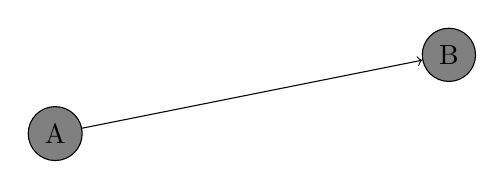
\begin{tikzpicture}
\node[draw, circle, fill=gray] at (0, 0) (A) {A};
\node[draw, circle, fill=gray] at (5, 1) (B) {B};
\draw [->] (A) -- (B);
\end{tikzpicture}

Scaler multiple 

Changes the length of the vectors, ie, stretches them in a direction. 

Length of k$\vec{v} =|K| * |V|$ 

direction of $k\vec{V} = same as \vec{V} if k > 0$

real numbers work like scaling factors 


\section{Chapter 13: vector functions}

\section{Chapter 14: partial derivate}

\section{Chapter 15: multiple integrals}

\section{Chapter 16: vector calculus}


\end{document}